\thispagestyle{myheadings} % should I be including this at the top of every section page??

\graphicspath{ {Body/Figures/TrackingFigures/} {Body/Figures/TrackingFigures/MainPlots/} {Body/Figures/TrackingFigures/MainPlots/PlanePlots/} {Body/Figures/TrackingFigures/MainPlots/PullPlots/} {Body/Figures/TrackingFigures/MainPlots/Residuals/} {Body/Figures/TrackingFigures/eLoss/} {Body/Figures/TrackingFigures/CoordSys/} {Body/Figures/TrackingFigures/TrackerPics/} {Body/Figures/TrackingFigures/Field/} {Body/Figures/TrackingFigures/TrackingFlow/} {Body/Figures/TrackingFigures/LeftRight/} {Body/Figures/TrackingFigures/Misc/}}


\chapter{Straw Tracking Analysis}
\label{chapter:Straw Tracking Analysis}

\section{Straw Tracking Intro}
\label{sec:StrawTrackingIntro}

As was talked about briefly in section \ref{sec:StrawTrackers}, the straw trackers are used to provide information about the muon beam, as well as info for the calorimeters. The straw track reconstruction is performed in several stages. The ``Track Finding'' stage takes incoming hits and decides which hits should be grouped together to form a single track for a single positron. The ``Track Fitting'' stage fits the measured positions of these invidividual hits and forms a single track describing the trajectory of the incident positron. Finally the ``Track Extrapolation'' stage takes the fitted track information and extrapolates the position and momentum components to the regions of interest, namely the storage region and the calorimeter.







-see the previous section for the hardware information...
-Geane (Geometry and Error Propagation)




\section{Track Finding}
\label{sec:Track Finding}

\section{Track Fitting}
\label{sec:Track Fitting}

The Geane fitting routines originated in Fortran with the EMC collaboration, and was used in the precursor E821 experiment as well as the PANDA experiment with some success \cite{geanemanual}, \cite{Lavezzi}. (I'm not actually aware of a useful reference for it's use in E821, and there are some other instances of its use as well in other experiments. In E821 there was a single tracking chamber which was never put to full use.) The core error propagation routines were at some point added to Geant4 under the error\_propagation directory which is included in all default installs. The tracking code strengths lie with its direct implementation and access to the Geant4 geometry and field, and its ability to handle the field inhomogeneties. The Geane fitting algorithm code which makes use of the Geant4 error propagation routines follows the structure of \cite{geanemanual} and is detailed in the \hyperref[sec:Formalism]{Formalism} section in this paper. It is a relatively straight forward least squares global \chisq minimization algorithm. 


Because of the proximity of the trackers to the muon beam, they will lie within a region of varying magnetic field. The radial field of the trackers rises from 0 Tesla at the outer ends to roughly .3 Tesla at the inner top and bottom ends, and the vertical field drops approximately 50\% from the storage dipole field of 1.451 Tesla. Shown in Figures \ref{fig:operaBy} and \ref{fig:operaBx} is the location of the tracker with respect to the horizontal and vertical fields respectively. These large field gradients over the tracking detector region and the long extrapolation distance back to the muon decay point are special to Muon \gmtwo. This is one of the main motivations for using the Geane fitting algorithm and routines, which has direct access to the field.

\begin{figure}[]
	\caption[Vertical magnetic field from Opera2D]{Shown is the vertical field of the \gmtwo magnet in and around the storage region as calculated in Opera 2D. The center of the storage region lies at 7.112 m along the x axis. The black box shows the rough location of the tracker with respect to the field (size exaggerated slightly). It can be seen that there is a large inhomogeneity within the tracker space, goring from left to right.}
	\centering
	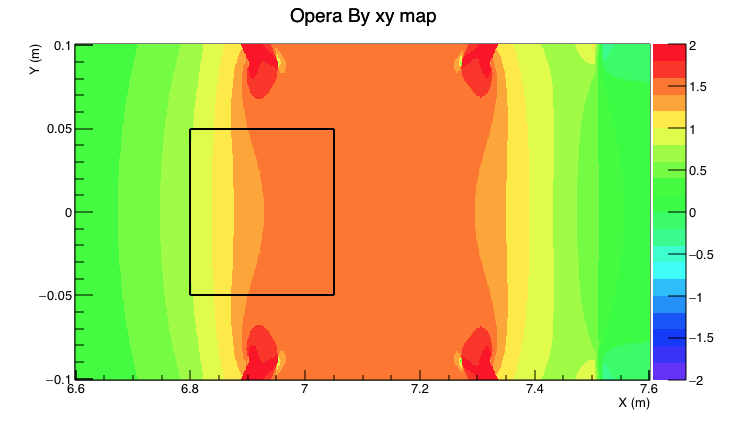
\includegraphics[width=0.9\textwidth]{operaBy}
	\label{fig:operaBy}
\end{figure}

\begin{figure}[]
	\caption[Horizontal magnetic field from Opera2D]{Shown is the radial field of the \gmtwo magnet in and around the storage region as calculated in Opera 2D. The center of the storage region lies at 7.112 m along the x axis. The black box shows the rough location of the tracker with respect to the field (size exaggerated slightly). It can be seen that there is a large homogeneity at the inner upper and lower ends compared to the right center. The shape of the pole pieces and tips can readily be seen.}
	\centering
	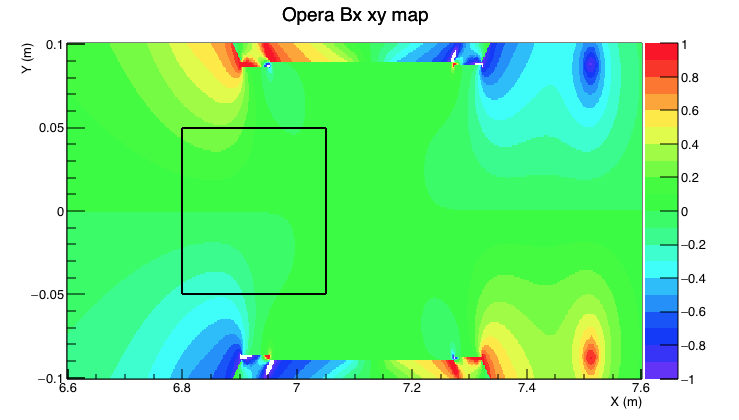
\includegraphics[width=0.9\textwidth]{operaBx}
	\label{fig:operaBx}
\end{figure}





\section{Track Extrapolation}
\label{sec:Track Extrapolation}
